% These are the lecture notes for my CSCI360 course SPRING 2017
% at John Jay College of Criminal Justice. They are based largely on
% Schneier's Applied Cryptography.

% Feel free to edit these slides and use them for your own courses.
% HOWEVER DO NOT REMOVE THESE LINES!
% Email me at: awood [at] jjay.cuny.edu
% or at: awood [at] gradcenter.cuny.edu


\documentclass{beamer}

\usepackage{tikz}
\usetikzlibrary{calc}

\usepackage{forest}
\usepackage{verbatim}
\usepackage{color}
\usepackage{amsmath}


\setbeamertemplate{footline}[frame number]
\setbeamertemplate{navigation symbols}{} 

\newtheorem{thm}{Theorem}[section]
\newtheorem{lem}{Lemma}
\newtheorem{cl}{Claim}
\newtheorem{cor}{Corollary}[section]
\newtheorem{conj}{Conjecture}
\newtheorem{quest}{Question}
\newtheorem{defn}{Definition}[section]
\newtheorem{obs}{Observation}[section]
\newtheorem{exam}{Example}

\newcommand{\im}{\operatorname{im}}
\newcommand{\id}{\operatorname{id}}
\newcommand{\interior}{\operatorname{int}}
\newcommand{\bdry}{\operatorname{bdry}}
\newcommand{\<}{\langle}
\renewcommand{\>}{\rangle}
\newcommand{\Gab}{(G_\phi)^{ab}} 
\newcommand{\phibar}{\bar{\phi}}
\newcommand{\Z}{\mathbb{Z}}
\newcommand{\N}{\mathbb{N}}
\newcommand{\Q}{\mathbb{Q}}
\newcommand{\R}{\mathbb{R}}
\newcommand{\C}{\mathbb{C}}
\newcommand{\A}{\mathcal{A}}
\newcommand{\OO}{\mathcal{O}}
\newcommand{\UU}{\mathcal{U}}
\newcommand{\power}{2^{\{P_1, \cdots , P_n\}}}
\newcommand{\bp}{\begin{problem}}
\newcommand{\ep}{\end{problem}}
\newcommand{\ba}{\begin{answer}}
\newcommand{\ea}{\end{answer}}
\newcommand{\ds}{\displaystyle}
\newcommand{\ben}{\renewcommand{\theenumi}{\alph{enumi}}
\renewcommand{\labelenumi}{(\theenumi)}\begin{enumerate}}
\newcommand{\een}{\end{enumerate}}
\newcommand{\Hess}{\operatorname{Hessian}}
\newcommand{\Aut}{\mathrm{Aut}}
\newcommand{\Inn}{\mathrm{Inn}}
\newcommand{\Out}{\mathrm{Out}}
\newcommand{\End}{\mathrm{End}}


\mode<presentation>
{
%  \usetheme{default}
  \setbeamercovered{invisible}
}


\usepackage[english]{babel}
\usepackage[latin1]{inputenc}
\usepackage{times}
\usepackage[T1]{fontenc}
\usepackage{stmaryrd}

%\usetheme{default}
%\usetheme{AnnArbor}
%\usetheme{Antibes}
%\usetheme{Bergen}
%\usetheme{Berkeley}
%\usetheme{Berlin}
%\usetheme{Boadilla}
%\usetheme{CambridgeUS}
%\usetheme{Copenhagen}
%\usetheme{Darmstadt}
%\usetheme{Dresden}
%\usetheme{Frankfurt}
%\usetheme{Goettingen}
%\usetheme{Hannover}
%\usetheme{Ilmenau}
%\usetheme{JuanLesPins}
%\usetheme{Luebeck}
%\usetheme{Madrid}
%\usetheme{Malmoe}
%\usetheme{Marburg}
%\usetheme{Montpellier}
%\usetheme{PaloAlto}
%\usetheme{Pittsburgh}
%\usetheme{Rochester}
\usetheme{Singapore}
%\usetheme{Szeged}
%\usetheme{Warsaw}

%\usecolortheme{default}
%\usecolortheme{albatross}
\usecolortheme{beaver}
%\usecolortheme{beetle}
%\usecolortheme{crane}
%\usecolortheme{dolphin}
%\usecolortheme{dove} % grey, white, yellow
%\usecolortheme{fly} %grey, yellow
%\usecolortheme{lily} %white, yellow, blue
%\usecolortheme{orchid}
%\usecolortheme{rose}
%\usecolortheme{seagull}
%\usecolortheme{seahorse}
%\usecolortheme{whale}
%\usecolortheme{wolverine}

% Title page

\title[OTP]{Perfect Secrecy and the One-Time Pad}

\subtitle{Based on \emph{Modern Cryptography} Katz \& Lindell Chapter 2}

\author
{Lecture notes of Alexander Wood \\ \scriptsize \href{mailto:awood@jjay.cuny.edu}{awood@jjay.cuny.edu}}
\institute[JJay]{John Jay College of Criminal Justice}  

\date{}

\begin{document}

% Remove 'figure' text from figure captions 
\setbeamertemplate{caption}{\raggedright\insertcaption\par}

\begin{frame}
  \titlepage
\end{frame}

\begin{frame}
\frametitle{The One-Time Pad}

\begin{columns}
\begin{column}{0.5\textwidth}
\begin{figure}
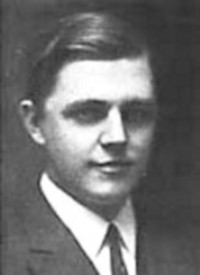
\includegraphics[scale=.5]{IMG/vernam}
\end{figure}
\end{column}
\begin{column}{0.5\textwidth}
Patented by Vernam in 1917.
\end{column}
\end{columns}
\end{frame}


\begin{frame}
\frametitle{Perfect Secrecy}

\begin{columns}
\begin{column}{0.4\textwidth}
In the 1940s Claude Shannon, the ``father of the information age,'' formulated a definition for \textbf{perfect secrecy}.
\end{column}
\begin{column}{0.5\textwidth}
\begin{figure}
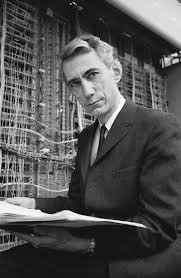
\includegraphics[scale=.7]{IMG/shannon}
\end{figure}
\end{column}
\end{columns}
\end{frame}


\begin{frame}
\frametitle{Perfect Secrecy, Informal}

Informally, \textbf{perfect secrecy} means that the ciphertext reveals \emph{no} knowledge about the underlying plaintext, and the adversary learns absolutely \emph{nothing} about the plaintext which was encrypted.
\end{frame}


\begin{frame}[fragile]
\frametitle{Perfect Secrecy, Formal}

\small
Now let's look at the formal definition of perfect secrecy provided in \emph{Introduction to Modern Cryptography} by Katz \& Lindell. \newline

\normalsize
\begin{defn}
An encryption scheme $(\verb|KeyGen|, \verb|Enc|, \verb|Dec|)$ with message space $\mathcal M$ is \textbf{perfectly secret} if for every probability distribution over $\mathcal M$, every message $m\in \mathcal M$, and every ciphertext $c\in\mathcal C$ for which $\Pr[C = c] >0$, 
\[
\Pr[M=m | C=c] = \Pr[M=m]
\]
\end{defn}
\end{frame}

\begin{frame}
\frametitle{Wait... what?}
\begin{figure}
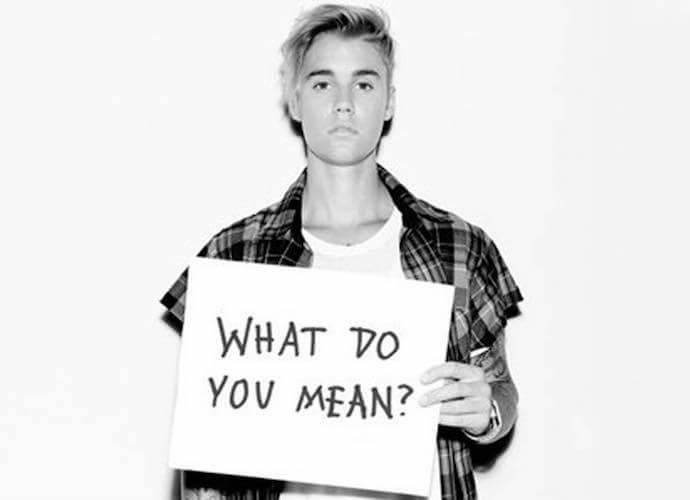
\includegraphics[scale=.3]{IMG/whatdoumean}
\end{figure}

Let's unpack this definition a bit.
\end{frame}


\begin{frame}
\frametitle{Message Space}

The \textbf{message space} $\mathcal M$ is a formal way of discussing the set of all \emph{possible} messages which could conceivably be sent. 
\end{frame}

\begin{frame}
\frametitle{Message Likelihood}

When we say that the adversary knows the probability distribution over the message space $\mathcal M$, we mean that \textbf{the adversary knows the likelihood that different messages are being sent}.
\end{frame}


\begin{frame}
\frametitle{What does the adversary know ?}

In the perfect secrecy model, the adversary knows:
\begin{itemize}
\item The likelihood that different messages will be sent
\item The encryption scheme
\end{itemize}

The only thing the adversary does \emph{not} know is the private key(s).
\end{frame}


\begin{frame}
\frametitle{Perfect Secrecy: The Game}

As before, thinking of perfect secrecy as a game can help us understand it better. The game proceeds as follows:
\begin{enumerate}
\item Alice chooses a message, encrypts it honestly, and sends it to Bob.
\item Eve eavesdrops on this message and receives the ciphertext $C$. 
\item Eve analyses the ciphertext. If Eve knows nothing more after her analysis about the ciphertext than she knew before, we say the scheme is perfectly secret.
\end{enumerate}
\end{frame}


\begin{frame}
\frametitle{Perfect Secrecy: Attack Model}

\emph{Which attack model does this fall under?} \newline

\pause

\begin{figure}
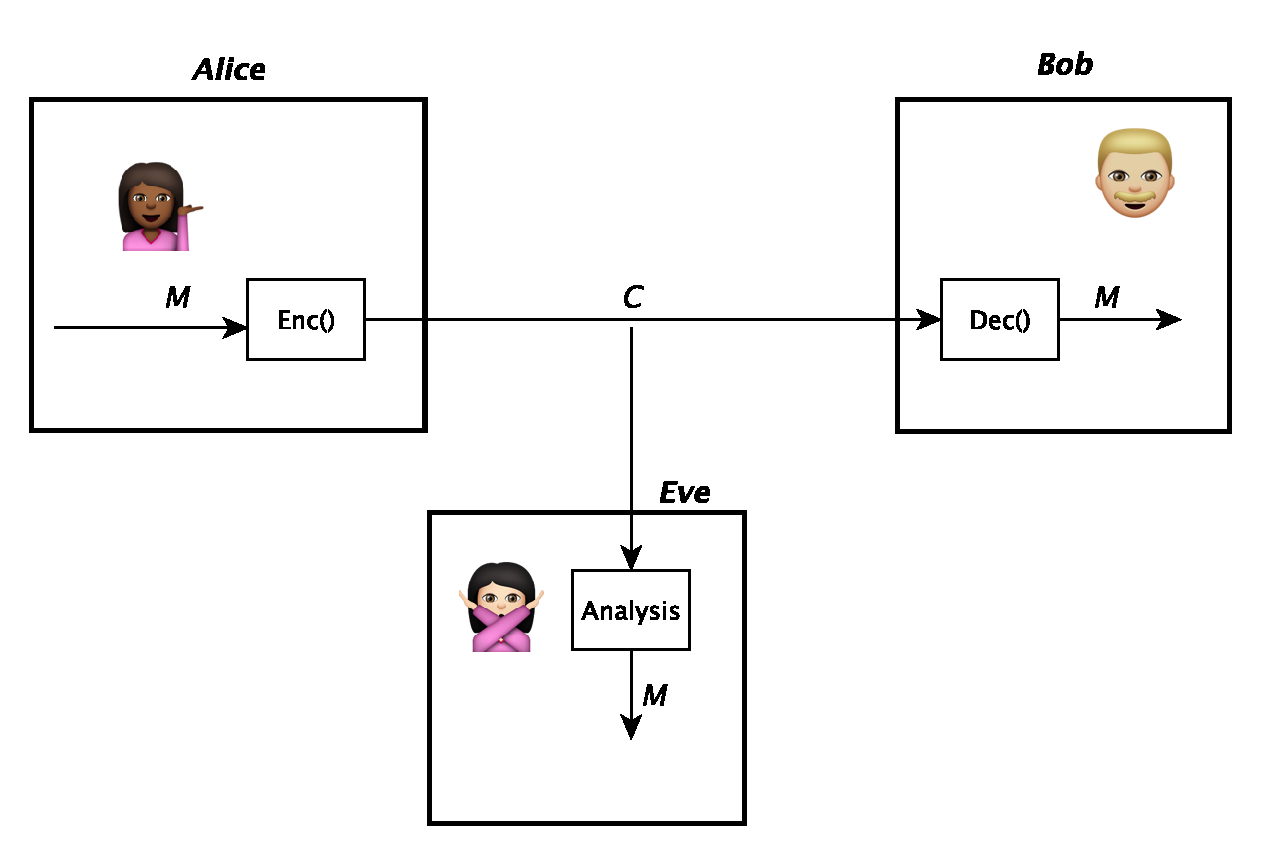
\includegraphics[scale=.3]{IMG/attack1}
\end{figure}
It is a ciphertext-only attack, since Eve only has access to the ciphertexts which she can eavesdrop on.
\end{frame}


\begin{frame}
\frametitle{Attack Model}

Here's another way of visualising the attack model.
\begin{figure}
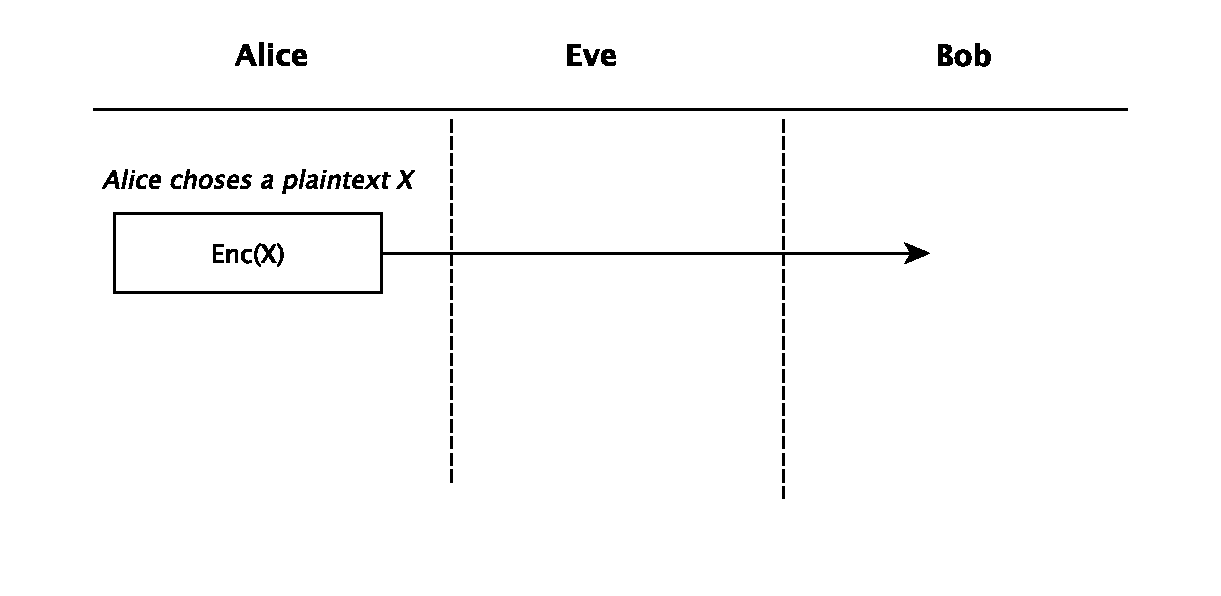
\includegraphics[scale=.5]{IMG/perfectsecrecy}
\end{figure}
\end{frame}



\begin{frame}
\frametitle{Perfect Secrecy}

When can we truly know that it is impossible for Eve to have learned \textbf{any information at all} about the message?
\end{frame}


\begin{frame}
\frametitle{Probability Distributions On Plaintext vs. Ciphertext}

For every two messages $m, m'\in\mathcal M$ and every ciphertext $c\in \mathcal C$,
\[
\Pr[Enc_K(m) = c] = \Pr[Enc_K(m') = c].
\]
This means that \textbf{it is impossible to distinguish an encryption of any message from an encryption of any other message.}
\end{frame}


\begin{frame}[fragile]
\frametitle{Non-example: Vigen\`{e}re}

Consider the the message space $\mathcal M$ which consists of all two-character strings, such as \verb|AB|, \verb|YY|, etc. Assume the keyspace consists of all one- or two-letter keys. \newline
\end{frame}




\begin{frame}
\frametitle{Non-example: Vigen\`{e}re}

Observe that
\[
\Pr[m = aa] = \frac{1}{26}\cdot \frac{1}{26}
\]
However,
\[
\Pr[m = aa | c = xy] = \frac{1}{2}\cdot\frac{1}{26}\cdot\frac{1}{26}
\]
\end{frame}



\begin{frame}[fragile]
\frametitle{The One-Time Pad Cryptosystem}

\begin{itemize}
\item \verb|KeyGen|: The key generation algorithm randomly generates a key $K$ as a binary string of length $n$.
\item \verb|Enc|: Represent the message $m$ as a binary string of length $n$. Encrypt via the bitwise XOR operation,
\[
c = K \oplus m.
\]
\item \verb|Dec| Decrypt by computing $m = K \oplus c$.
\end{itemize}
\end{frame}

\begin{frame}
\frametitle{The One-Time Pad Cryptosystem}

\begin{figure}
\includegraphics[scale=.55]{IMG/otp}
\end{figure}
\end{frame}


\begin{frame}[fragile]
\frametitle{Representing Characters As Bits}

Each ASCII character can be converted to a bit string of length 8 (one byte). For instance,
\[
\verb|'A'| = 65
\]
and
\[
65 = [01000001]_2
\]
\end{frame}


\begin{frame}
\frametitle{Characters to Bits and Back in Python}

\begin{columns}
\begin{column}{0.5\textwidth}
\textbf{Characters to bits:}
\begin{figure}
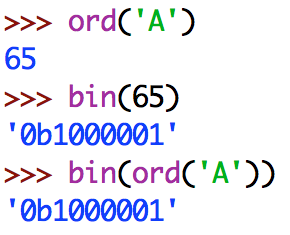
\includegraphics[scale=.7]{IMG/py}
\end{figure}
\end{column}
\begin{column}{0.5\textwidth}
\textbf{Bits to characters:}
\begin{figure}
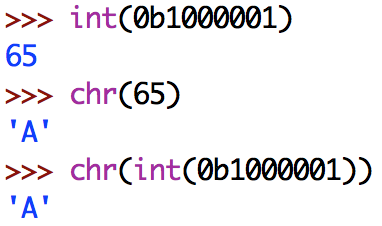
\includegraphics[scale=.7]{IMG/py2}
\caption{or specify base with string input:}
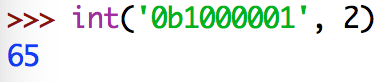
\includegraphics[scale=.6]{IMG/py3}
\end{figure}

\end{column}
\end{columns}
\end{frame}

\begin{frame}[fragile]
\frametitle{Coding Exercise 1: Characters To Bitstrings}

\begin{verbatim}
INPUT: A string of characters.
OUTPUT: A bitstring, where each 8 bits 
        corresponds to the letters in the string.

Example:
INPUT: 'A'
OUTPUT: '01000001'

INPUT: 'AA'
OUTPUT: '0100000101000001'

INPUT: 'AB'
OUTPUT: '0100000101000010'
\end{verbatim}
\end{frame}


\begin{frame}[fragile]
\frametitle{Coding Exercise 2: Bits To Characters}
\begin{verbatim}
INPUT: A bit string.
OUTPUT: A string of the characters 
        encoded by the bit string. 

Example:
INPUT: '01000001'
OUTPUT: 'A'

INPUT: '0100000101000010'
OUTPUT: 'AB'
\end{verbatim}
\end{frame}

\begin{frame}[fragile]
\frametitle{Encrypting with XOR}

A message \verb|01000001| would be encoded with the One-Time Pad using secret key \verb|10110101| using \verb|XOR| (exclusive-or) as follows:
\begin{verbatim}
Message:    01000001
Key:        10110101

XOR:        11110100
\end{verbatim}
\end{frame}


\begin{frame}
\frametitle{OTP And Perfect Secrecy}

We want to convince ourselves that encryption using the One-Time Pad does \emph{nothing} to give away \emph{any} information about the plaintext message. 
\end{frame}


\begin{frame}
\frametitle{OTP And Perfect Secrecy}

Consider trying a brute-force attack on the OTP system. If the message is $b$ bits long, there are $2^b$ possible keys. However, there are also $2^b$ possible messages. \newline

Any ciphertext message of length $b$ could possibly decrypt to \emph{any} plaintext message of length $b/8$ (post-conversion from bytes to chars). \newline

The OTP gives us nothing else to work with! The encryption is no more likely to be one message than literally any other message of that length. 
\end{frame}


\begin{frame}[fragile]
\frametitle{Why Use XOR?}

Why use \verb|XOR|, instead of \verb|AND| or \verb|OR|?\newline

\begin{columns}
\begin{column}{.3\textwidth}
\begin{tabular}{ r|c|c| }
\multicolumn{1}{r}{}
 &  \multicolumn{1}{c}{0}
 & \multicolumn{1}{c}{1} \\
\cline{2-3}
0 &  0&  1\\
\cline{2-3}
1 & 1&0 \\
\cline{2-3}
\end{tabular}\newline

\verb|    XOR|
\end{column}
\begin{column}{.3\textwidth}
\begin{tabular}{ r|c|c| }
\multicolumn{1}{r}{}
 &  \multicolumn{1}{c}{0}
 & \multicolumn{1}{c}{1} \\
\cline{2-3}
0 &  0&  1\\
\cline{2-3}
1 &1 & 1\\
\cline{2-3}
\end{tabular}\newline

\verb|    OR|
\end{column}
\begin{column}{.3\textwidth}
\begin{tabular}{ r|c|c| }
\multicolumn{1}{r}{}
 &  \multicolumn{1}{c}{0}
 & \multicolumn{1}{c}{1} \\
\cline{2-3}
0 &  0& 0 \\
\cline{2-3}
1 &0 & 1\\
\cline{2-3}
\end{tabular}\newline

\verb|    AND|
\end{column}
\end{columns}
\vspace{5mm}

The \verb|XOR| gate is the only one which is equally likely to have \verb|0| or \verb|1| as an output. 
\end{frame}


\begin{frame}
\frametitle{Why Use XOR?}
Let's look at the illustrations on Khan Academy at the following link to visualize this.\newline

\url{https://www.khanacademy.org/computing/computer-science/cryptography/ciphers/a/xor-and-the-one-time-pad}
\end{frame}


\begin{frame}[fragile]
\frametitle{Why a ONE-time Pad?}

Assume Alice has two messages, $m_1$ and $m_2$, and a key $k$. She sends
\[
c_1 = m_1 \oplus k \text{ and } c_2 = m_2 \oplus k
\]
to Bob. Now, an eavesdropper Eve can compute 
\[
c_1 \oplus c_2 = (m_1\oplus k) \oplus (m_2\oplus k) = m_1 \oplus m_2
\]
Eve can't necessarily find $m_1$ or $m_2$, but she can find the \verb|XOR| of the plaintexts. Thus she has reduced her work from finding two messages $m_1$ and $m_2$ to finding only one message, since she has found a dependence between them.\newline

Successful hacks of the ``many-time'' pad have been carried out by cryptographers. 
\end{frame}


\begin{frame}
\frametitle{OTP: Practical?}

\textbf{If the One-Time Pad is perfectly secure, why is not used for everything?!}\newline

\pause

The problem is key distribution. Once the key is distributed, the one-time pad can satisfy perfect secrecy. In real-life applications, the One-Time Pad is only as secure as the key distribution method. 
\end{frame}


\begin{frame}[fragile]
\frametitle{Coding Exercise 3: Key Generation Algorithm}

\begin{verbatim}
INPUT: Integer n, the desired length of the key.
OUTPUT: The key, a bit string of length n. 

Hint: use random.randint(0,1)

Example:
INPUT: 8
OUTPUT: 10101111

INPUT: 8
OUTPUT: 01101001

INPUT: 16
OUTPUT: 001011101001010
\end{verbatim}
\end{frame}

\begin{frame}
\frametitle{References}

\begin{itemize}
\item \emph{Modern Cryptography} by Katz \& Lindell Chapter 2
\item emph{Hacking Secret Ciphers With Python} Chapter 22
\item Khan Academy: \url{https://www.khanacademy.org/computing/computer-science/cryptography/crypt/v/one-time-pad}
\end{itemize}
\end{frame}
\end{document}


